\section{Auswertung}
\label{sec:Auswertung}
Zuerst wird der Energieverlust der Alphateilchen bestimmt. Dieser wird ermittelt, 
indem die Energie der Teilchen gegen die effektive Weglänge aufgetragen wird. 
Die effektive Weglänge wird dabei mithilfe von Formel (\ref{eqn:effektive_Laenge}) berechnet. 
Die Energie wird durch einfachen Dreisatz aus mehreren Informationen berechnet. Zum einen ist wichtig, dass
die Energie proportional zum Channel, indem die meisten Teilchen gemessen werden, ist und zum anderen, dass
der Channel, indem bei einem Druck von $0 \, \unit{\milli\bar}$ die meisten Teilchen sind,
eine Energie von $4 \, \unit{\mega\eV}$ hat. Die Anzahl der Teilchen, 
die abhängig vom Druck gemessen werden und die Channel, in denen die meisten Teilchen gezählt
werden, sind in Tabelle (\ref{tab:Abstand_1}) für einen Abstand der Probe von $x_{0,1}= 4,5 \, \unit{\centi\meter}$ und in Tabelle (\ref{tab:Abstand_2}) 
für einen Abstand der Probe von $x_{0,2} = 6 \, \unit{\centi\meter}$ aufgelistet. 

\begin{table}[H]
    \centering
    \caption{Eingestellter Druck, gemessene Pulsanzahl und Channel mit der höchsten Pulsrate bei einem Abstand von 4,5 cm}
    \label{tab:Abstand_1}
    \begin{tblr}{colspec={c c c}}
        \toprule
        $\text{Druck} \, \left[\unit{\milli\bar}\right]$ & $\text{Anzahl der gemessenen Pulse}$ &  $\text{Channel der maximalen Pulszahl}$ \\
        \midrule
        0   & 26225 & 1239 \\
        60  & 26012 & 1158 \\
        100 & 25800 & 1064 \\
        150 & 25502 & 999 \\
        200 & 25299 & 926 \\
        260 & 24468 & 839 \\
        300 & 24326 & 770 \\
        350 & 23974 & 720 \\
        400 & 22682 & 620 \\
        450 & 21331 & 511 \\
        500 & 15645 & 423 \\
        560 & 1433  & 415 \\
        \bottomrule
    \end{tblr}
\end{table}

\begin{table}[H]
    \centering
    \caption{Eingestellter Druck, gemessene Pulsanzahl und Channel mit der höchsten Pulsrate bei einem Abstand von 6 cm}
    \label{tab:Abstand_2}
    \begin{tblr}{colspec={c c c}}
        \toprule
        $\text{Druck} \,  \left[\unit{\milli\bar}\right]$ & $\text{Anzahl der gemessenen Pulse}$ &  $\text{Channel der maximalen Pulszahl}$ \\
        \midrule
        0 & 16038 & 1171 \\
        50 & 15679 & 1109 \\
        100 & 15145 & 995 \\
        150 & 15031 & 921 \\
        200 & 14814 & 839 \\
        250 & 14313 & 775 \\
        300 & 13741 & 640 \\
        350 & 13076 & 614 \\
        400 & 6313 & 415 \\
        450 & 376 & 410 \\
        500 & 0 & 0 \\
        \bottomrule
    \end{tblr}
\end{table}

Die sich aus den Daten ergebenden Werte sind in Abbildung (\ref{fig:Abstand_1}) für den Abstand von $4,5 \, \unit{\centi\meter}$ und in Abbildung (\ref{fig:Abstand_2}) für den Abstand 
von $6 \, \unit{\centi\meter}$ geplottet. Dazu wird jeweils eine lineare Ausgleichsgerade der Form $y = mx + n$ aufgestellt und geplottet. 

\begin{figure}[H]
  \centering
  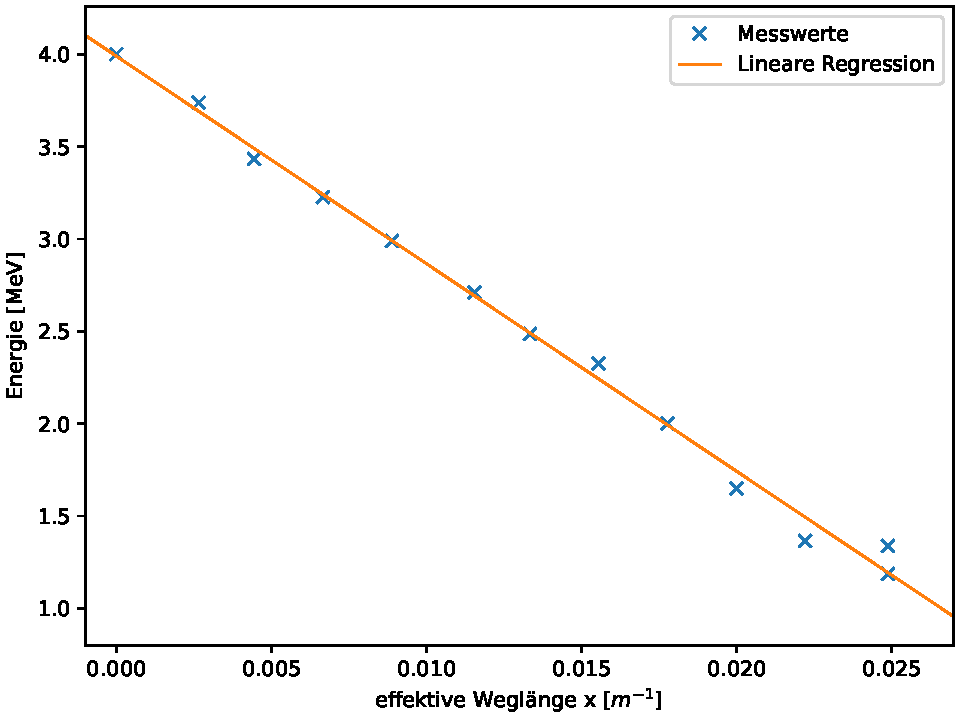
\includegraphics[width =0.75\textwidth]{Plots/plot1.pdf}
  \caption{Energie aufgetragen gegen die effektive Weglänge bei einer absoluten Entfernung von 4,5 cm mit Ausgleichsgerade}
  \label{fig:Abstand_1}
\end{figure}

\begin{figure}[H]
    \centering
    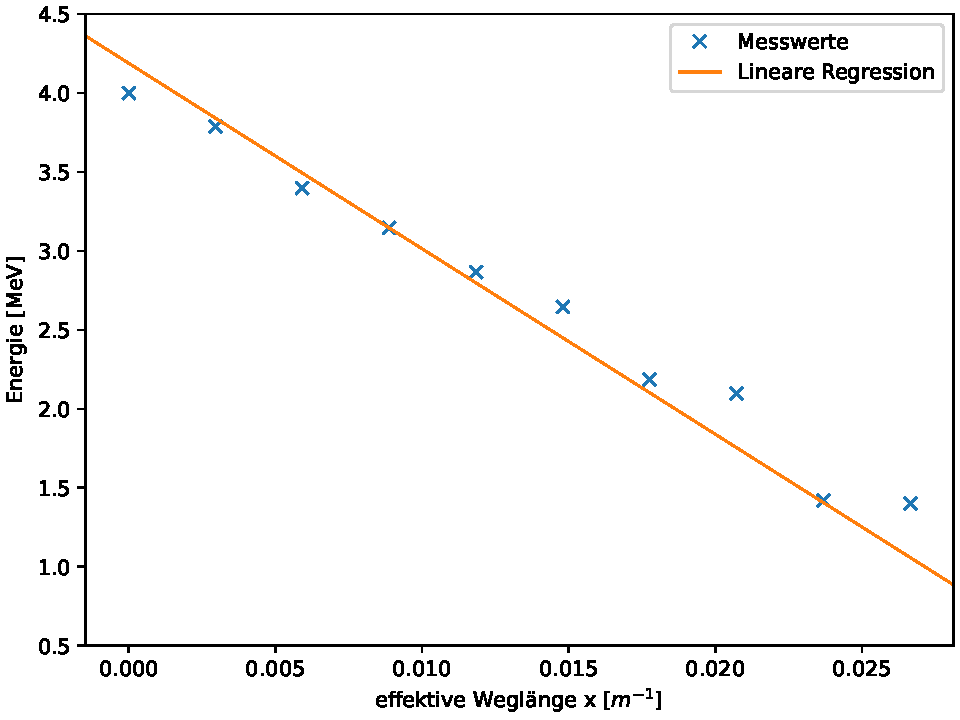
\includegraphics[width=0.75\textwidth]{Plots/plot2.pdf}
    \caption{Energie aufgetragen gegen die effektive Weglänge bei einer absoluten Entfernung von 6 cm mit Ausgleichsgerade}
    \label{fig:Abstand_2}
\end{figure}

Die Steigung der Ausgleichsgerade ist dabei der Energieverlust. Dieser beträgt bei einem Abstand von $4,5 \, \unit{\centi\meter}$ $m_1 = (-112 \pm 2,5)\, 
\unit[per-mode=fraction]{\mega\eV\per\meter}$. Bei einem Abstand von $6 \, \unit{\centi\meter}$ beträgt dieser $m_2 = (-117 \pm 9,8)\, 
\unit[per-mode=fraction]{\mega\eV\per\meter}$. 

Zur Bestimmung der mittleren Reichweite wird die gemessene Pulsanzahl gegen die effektive Weglänge aufgetragen und dann der Schnittpunkt der Ausgleichsgerade, 
die durch den zu sehenden starken Abfall geht und einer Konstanten bei der Hälfte der höchsten gemessenen Pulszahl. Dieser Schnittpunkt wird grün markiert. 
Der Plot zu einer Entfernung von $4,5 \, \unit{\centi\meter}$ ist Abbildung (\ref{fig:Weglaenge_1}) und zu einer Entferung von $6 \, \unit{\centi\meter}$ 
ist Abbildung (\ref{fig:Weglaenge_2}). 

\begin{figure}[H]
    \centering
    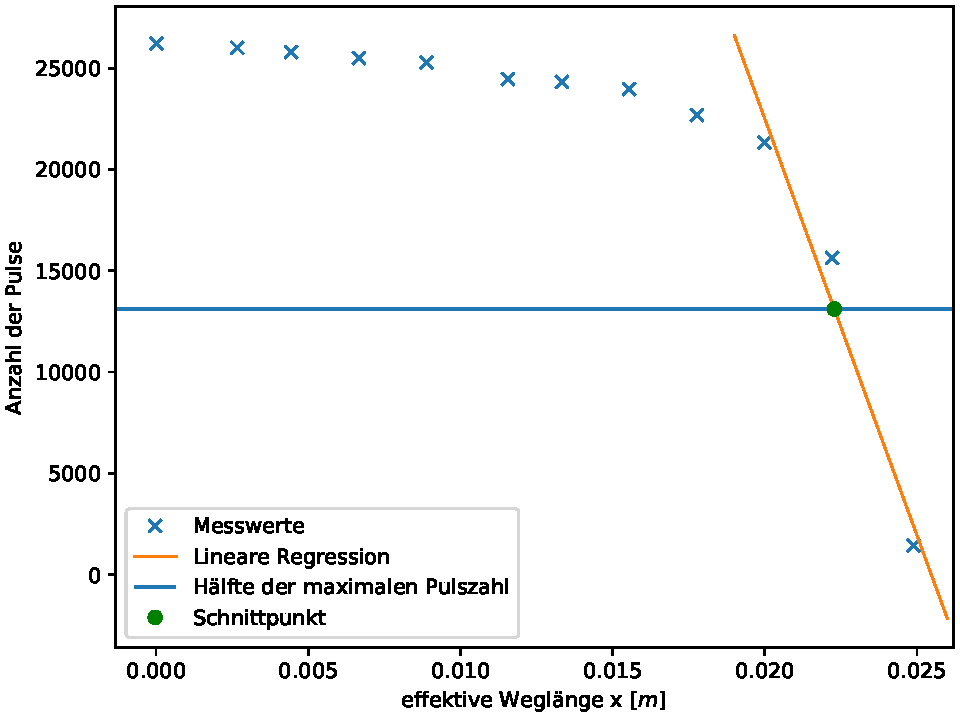
\includegraphics[width=\textwidth]{Plots/plot3.pdf}
    \caption{Pulsanzahl aufgetragen gegen die effektive Weglänge bei einer absoluten Entfernung von 4,5 cm}
    \label{fig:Weglaenge_1}
\end{figure}

\begin{figure}[H]
    \centering
    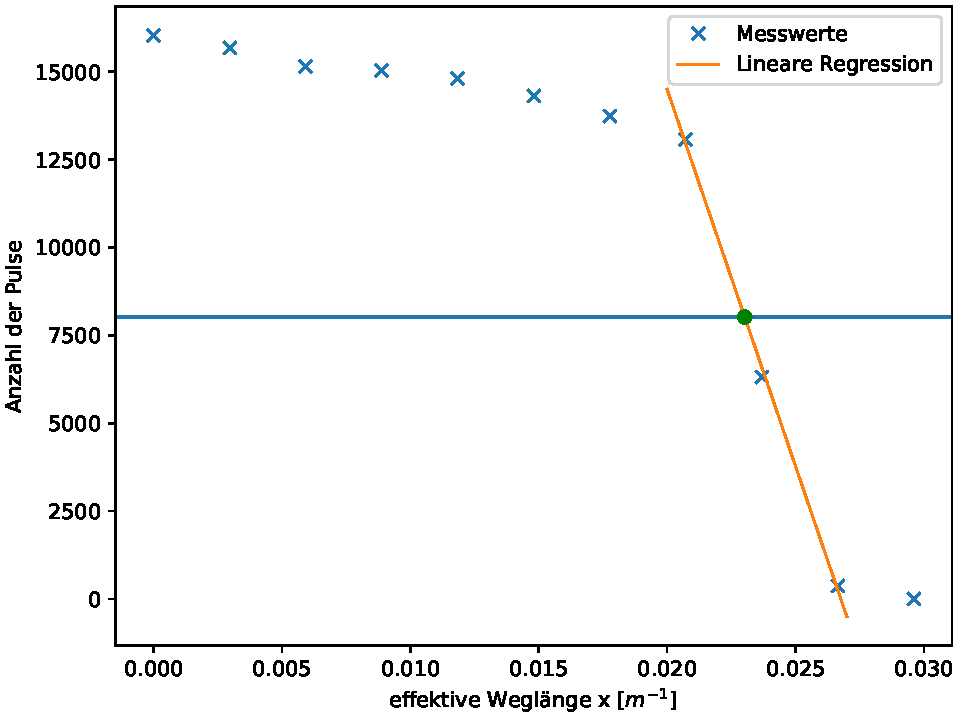
\includegraphics[width=\textwidth]{Plots/plot4.pdf}
    \caption{Pulszahl aufgetragen gegen die effektive Weglänge bei einer absoluten Entfernung von 6 cm}
    \label{fig:Weglaenge_2}
\end{figure}
Die x-Koordinate des grün markierte Schnittpunkts gibt die mittlere Reichweite an. Bei einer Entfernung von $4,5 \, \unit{\centi\meter}$ ist die mittlere Reichweite 
$x_1 = 2,26 \, \unit{\centi\meter}$ und bei einer Entfernung von $6 \, \unit{\centi\meter}$ ist diese $x_2 = 2,30 \, \unit{\centi\meter}$. 

Anschließend wird die statistische Messung, in der 100 Mal die Pulsanzahl in einem Zeitintervall von $10 \, \unit{\second}$ bei gleichem Druck und gleichem Abstand gemessen werden, mit einer Poissonverteilung und 
einer Gaußverteilung verglichen. Die gemessenen Pulszahlen sind in Tabelle (\ref{tab:Statistik}) zu sehen. 

\begin{table}[H]
    \centering
    \caption{Statistische Messung der Pulsanzahl in einem Zeitintervall von $10 \, \unit{\second}$}
    \label{tab:Statistik}
    \begin{tblr}{colspec={c c c c c c}}
        \toprule
        $\text{Pulsanzahl}$ & $\text{Pulsanzahl}$ & $\text{Pulsanzahl}$ & $\text{Pulsanzahl}$ & $\text{Pulsanzahl}$ & $\text{Pulsanzahl}$\\
        \midrule
        1338 & 1229 & 1205 & 1252 & 1154 & 1325 \\ 
        1233 & 1171 & 1336 & 1251 & 1241 & 1212 \\ 
        1246 & 1300 & 1215 & 1306 & 1298 & 1308 \\ 
        1329 & 1177 & 1176 & 1254 & 1158 & 1250 \\ 
        1161 & 1253 & 1307 & 1158 & 1189 & 1187 \\ 
        1209 & 1220 & 1189 & 1227 & 1249 & 1197 \\ 
        1235 & 1319 & 1204 & 1272 & 1175 & 1268 \\ 
        1272 & 1285 & 1188 & 1196 & 1323 & 1308 \\ 
        1222 & 1233 & 1246 & 1204 & 1236 & 1243 \\ 
        1225 & 1175 & 1289 & 1301 & 1141 & 1248 \\ 
        1315 & 1188 & 1260 & 1249 & 1267 & 1280 \\ 
        1293 & 1227 & 1241 & 1262 & 1307 & 1278 \\ 
        1284 & 1295 & 1292 & 1220 & 1244 & 1345 \\ 
        1270 & 1205 & 1258 & 1258 & 1227 & 1347 \\ 
        1316 & 1195 & 1219 & 1230 & 1196 & 1117 \\ 
        1208 & 1188 & 1225 & 1211 & 1312 & 1244 \\ 
        1218 & 1212 & 1271 & 1142 &      &  \\ 
        \bottomrule
    \end{tblr}
\end{table}
Diese Werte werden in Abbildung (\ref{fig:Gauss}) zusammen mit einer Gaußverteilung und dem oberen bzw. unterem Ende des Messdatenfehlers durch Histogramme
verschiedener Bingrößen dargestellt. 
\begin{figure}[H]
    \centering
    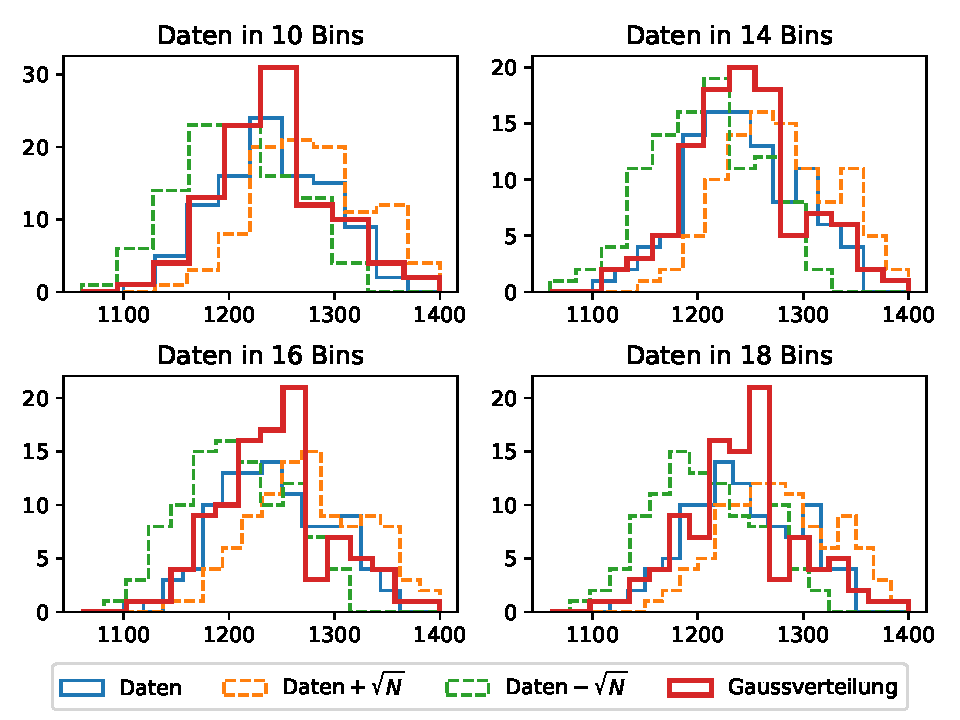
\includegraphics[width=\textwidth]{Plots/plot5.pdf}
    \caption{Histogramme mit verschiedenen Bingrößen zur Darstellung der Daten und der Gaußverteilung.}
    \label{fig:Gauss}
\end{figure}
In Abbildung (\ref{fig:Poisson}) sind die Daten zusammen mit einer Poissonverteilung dargestellt, um einen Vergleich zwischen Gauß- und Poissonverteilung möglich 
zu machen.
\begin{figure}[H]
    \centering
    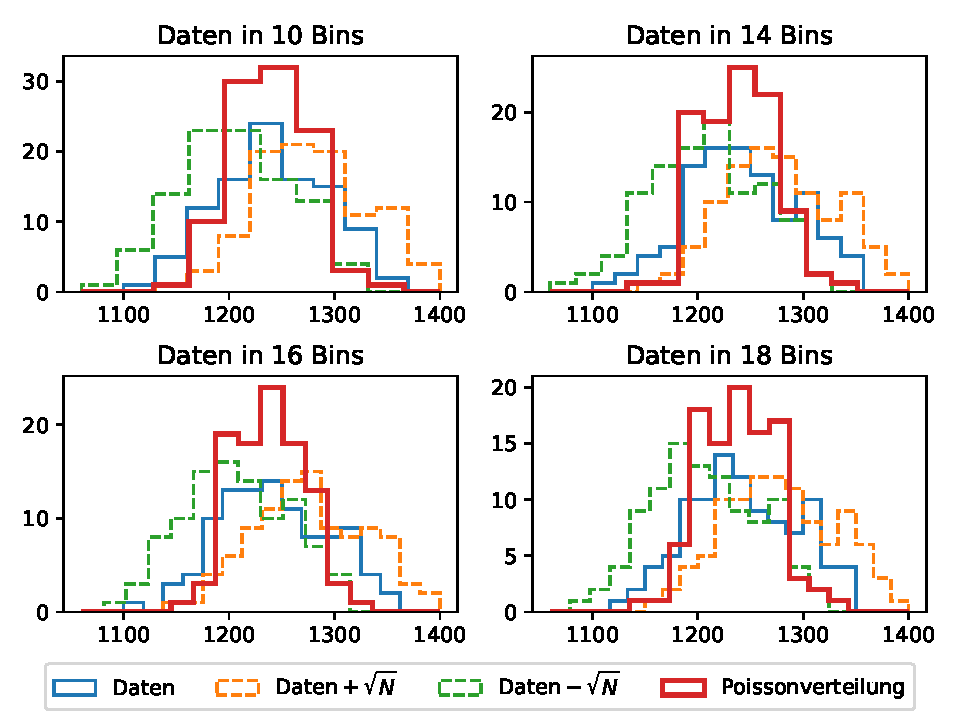
\includegraphics[width=\textwidth]{Plots/plot6.pdf}
    \caption{Histogramme mit verschiedenen Bingrößen zur Darstellung der Daten und der Poissonverteilung.}
    \label{fig:Poisson}
\end{figure}
Die verwendete Standardabweichung der Daten entspricht $51,48$ und der verwendete Mittelwert ist $1242 \pm 3,5 $. 
%Siehe \autoref{fig:plot}!